\documentclass[tikz,border=10pt]{standalone}
\usepackage{tikz}[scale=1, every node/.style={circle, draw, minimum size=5mm, inner sep=0pt}, >=Stealth]
\usepackage{pgffor}

\begin{document}
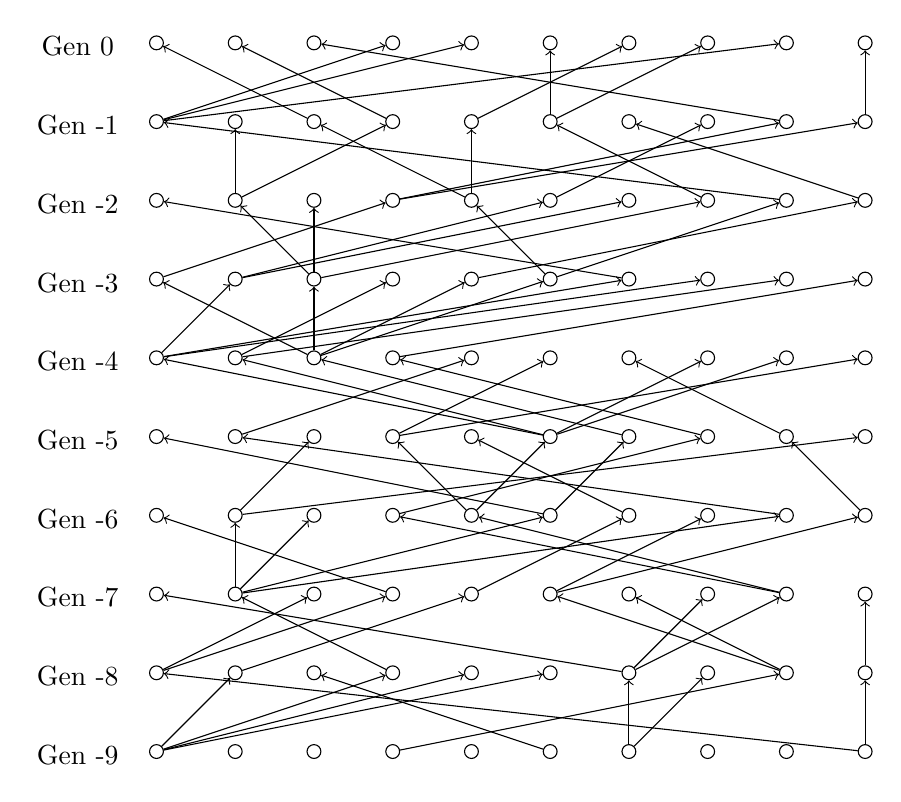
\begin{tikzpicture}
    \pgfmathsetseed{888}
    % Population size and number of generations
    \def\popsize{10} % Population size per generation
    \def\generations{10} % Number of generations
    \def\xspacing{1} % 横向间距
    \def\yspacing{1} % 纵向间距

    % Node coordinates
    \foreach \g in {1,...,\generations} {
        \foreach \i in {1,...,\popsize} {
            % Define nodes as "gen-g-i" where g = generation, i = individual
            \node[draw, circle, minimum size=5pt, inner sep=0pt] (gen-\g-\i) at (\i*\xspacing, -\g*\yspacing) {};
        }
    }

    % Arrows for ancestry
    \foreach \g in {2,...,\generations} {
        \pgfmathsetmacro{\prev}{int(\g - 1)} % Previous generation
        \foreach \i in {1,...,\popsize} {
            % Generate a random parent index in the range [1, \popsize]
            \pgfmathtruncatemacro{\ancestor}{rnd * \popsize + 1} % Scale and truncate to [1, \popsize]            
            % Draw an arrow from parent to current individual
            %\draw[->, color = gray] (gen-\g-\ancestor) -- (gen-\prev-\i);
            \draw[->] (gen-\g-\ancestor) -- (gen-\prev-\i);
        }
    }

    % Generation labels
    \foreach \g in {1,...,\generations} {
        \pgfmathsetmacro{\tracenum}{int(1-\g)}
        \node[below] at (0, -\g*\yspacing+0.2) {Gen \tracenum};
    }

    %for 123 seed
    \iffalse
    \foreach \g/\ancestor/\i in {2/1/2,2/6/5,2/7/7,2/10/8,3/3/1,3/5/6,3/5/7,3/6/10, 4/6/3,4/1/5,4/5/6, 5/6/6,5/9/1,5/9/5, 6/5/6,6/10/9, 7/6/5,7/4/10, 8/1/6,8/9/4, 9/4/1,9/4/9, 10/3/4}{
        \pgfmathsetmacro{\prev}{int(\g - 1)}
        \node[draw, circle, minimum size=5pt, inner sep=0pt] (gen-\prev-\i) at (\i*\xspacing, -\prev*\yspacing) {};
        \draw[very thick, ->,color = red] (gen-\g-\ancestor) -- (gen-\prev-\i);
    }
    \foreach \i/\l in {2/x,5/y,7/z,8/w}{
        \node[] (label-\i) at (\i*\xspacing, -1*\yspacing+0.25) {$\l$};
    }
\fi

%for 888 seed
\iffalse
\foreach \g/\ancestor/\i in {
    2/3/1,2/9/3,2/1/5,2/5/7,
    3/5/3,3/4/9,3/9/1,3/5/5, 
    4/6/5,4/1/4,4/6/9, 
    5/3/1,5/3/6, 
    6/7/3, 
    7/6/7, 
    8/2/6, 
    9/4/2, 
    10/1/4}{
        \pgfmathsetmacro{\prev}{int(\g - 1)}
        \node[draw, circle, minimum size=5pt, inner sep=0pt] (gen-\prev-\i) at (\i*\xspacing, -\prev*\yspacing) {};
        \draw[very thick, ->,color = red] (gen-\g-\ancestor) -- (gen-\prev-\i);
    }
    \foreach \i/\l in {1/x,3/y,5/z,7/w}{
        \node[] (label-\i) at (\i*\xspacing, -1*\yspacing+0.25) {$\l$};
    }
        \fi
\end{tikzpicture}
\end{document}